\documentclass{report}
\usepackage[utf8]{inputenc}
\title{Proyecto final:\\
Redes de computadoras}
\author{Olea Olvera Marco\\
Barocio Gomez Luis Fernando\\
Arteaga Hernandez Alejandro}
\date{Diciembre 2019}

\usepackage{natbib}
\usepackage{graphicx}
\usepackage[table,xcdraw]{xcolor}

\begin{document}

\maketitle

\section{Objetivo}
¡La aplicación que revolucionará la manera en que experimentamos pokemon!\\
Desarrollado en el lenguaje de programación del momento, utilizado para una gran cantidad de aplicaciones de manejo de datos, python.
\\\\
Es una aplicación portable 100\%, eso significa que puede correr sobre cualquier sistema o cualquier sistema operativo.
\\\\
El servidor soporta múltiples conexiones de diversos clientes, y al manejar hilos, es muy robusto, si una conexión tuviera algún error de comunicación, las demás seguirian estan sin problemas. 
\\\\
Tiene, un modo de debug, para que los desarrolladores posteriores puedan agregar nuevas funcionalidades, además de que también maneja códigos de error, y no permite códigos incorrectos, 
\\\\
El servidor cuenta con tiempos de esperar máximos, (Timeouts), si no se recibe una respuesta del cliente, la conexión se cerrará de manera correcta informando al cliente.
\\\\
El servidor cuenta con persistencia. Usa el manejador de datos SQLite3
es un manejador de datos Portable, eso significa que llevar la base de datos contigo a otro sistema es muy fácil, cuenta con un archivo llamado db.py en el cual ya vienen implementadas las consultas más frecuentes a la base de datos lo que hace muy fácil acceder a esos datos.\\\\
Además la aplicación guarda un registro con todas las capturas hechas por cada usuario, lo que permite que tu progreso se guarde. 
\\\\
Como se usó un manejador de datos robusto, la aplicación es muy cuidadosa de los datos que hace uso, además de que permite concurrencia e integridad de los datos y es facilmente portable a otro manejador de base de datos si así se requiere.\\\\

Y por último, la aplicación está desarrollada muy eficientemente, usa principios de ingeniería de software para hacer que el software sea altamente mantenible, debido a que está programado en módulos específicos que cada uno tiene una función, es muy extensible, si en el futuro se desean agregar funcionalidades. Cuenta con toda la documentación necesaria y cumple con buenos hábitos de programación.

\section{Diseño del protocolo}

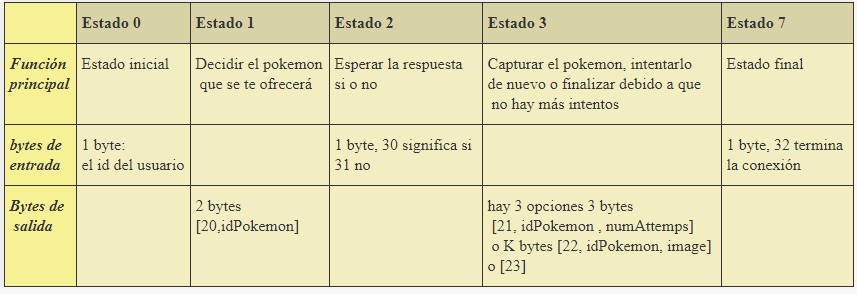
\includegraphics[scale=0.65]{tabla.PNG}
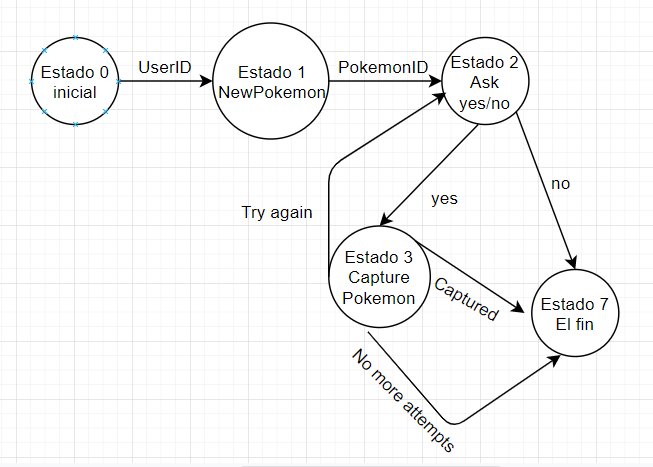
\includegraphics[scale=0.8]{flow.PNG}
\newpage
\section{Instrucciones de uso}
Para ejecutar necesitas tener python3 instalado\\
Las librerías socket e Image en algunas versiones es PIL
usar pip para instalarlas
\\\\
Para ejecutar el server entrar a la carpeta server y ejecutar\\
python ThreadedServer.py
\\\\\

Para ejecutar el cliente entrar a la carpeta cliente y ejecutar\\
python Client.py
\\\\\
en host poner el host deseado e igual en puerto, 
si quiere que se use localhost por defecto y el puerto 9999 
dejar en blanco cuando se pregunte\\\\
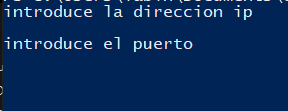
\includegraphics[scale=0.8]{introduce.PNG}
\section{Flujo del programa}
\begin{itemize}
    \item El primer paso para iniciar, debemos correr el Servidor,
    en el script ThreadedServer.py como su nombre lo indica es un servidor que lanza un hilo por cada conexión que genera\\
    Esto hará que se monte un servidor y que se ponga a escuchar la dirección 127.0.0.1 osea localhost en el puerto 9999.\\\\
      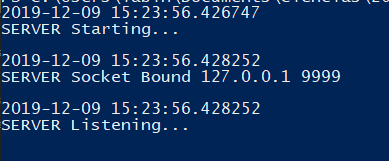
\includegraphics[scale=0.8]{inicioServer.PNG}
    
    \item El siguiente paso es iniciar el Cliente en la carpeta client, ejecutar el script Client.py, al iniciar este nos pedirá el host al que conectarse y el puerto, los ingresamos, si no ingresamos nada, se pondrá por defecto, localhost y el puerto 9999\\\\
    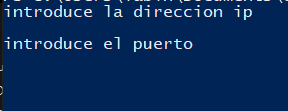
\includegraphics[scale=0.8]{introduce.PNG}
    
    \item Una vez que se ha configurado el cliente, el cliente hará una conexión con el servidor, el cual el servidor nos indicará con la siguiente linea\\\\
    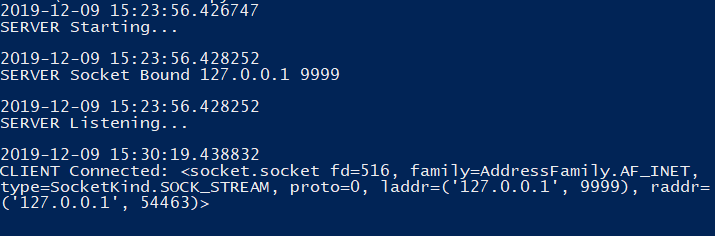
\includegraphics[scale=0.8]{conectado.PNG}
    \\\\Como se puede ver en la imagen estamos conectados via el localhost y la conexión del cliente sale del puerto 54463
    
    \item Una vez conectados comienza la aplicación
    Solo necesitas seguir el flujo que la consola te indique y será el que se mostró cuando puse la máquina de estados\\\
    La imagen capturada se mostrará con el selector de fotos de tu sistema operativo automáticamente\\\\
    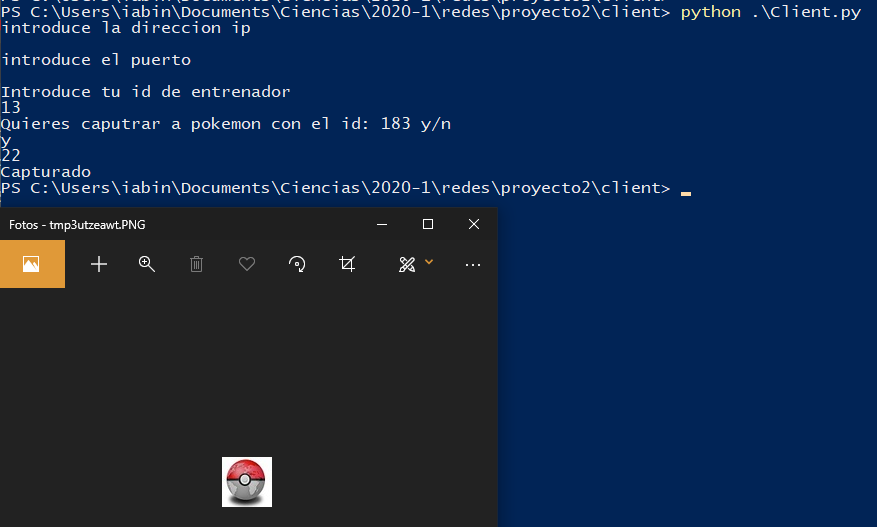
\includegraphics[scale=0.8]{capturado.PNG}
    \\\\
    De igual manera puede que te tomes mas intentos en capturar, o que trás 3 intentos no logres capturar el pokemon y la conexión se cerrará\\\\
    
    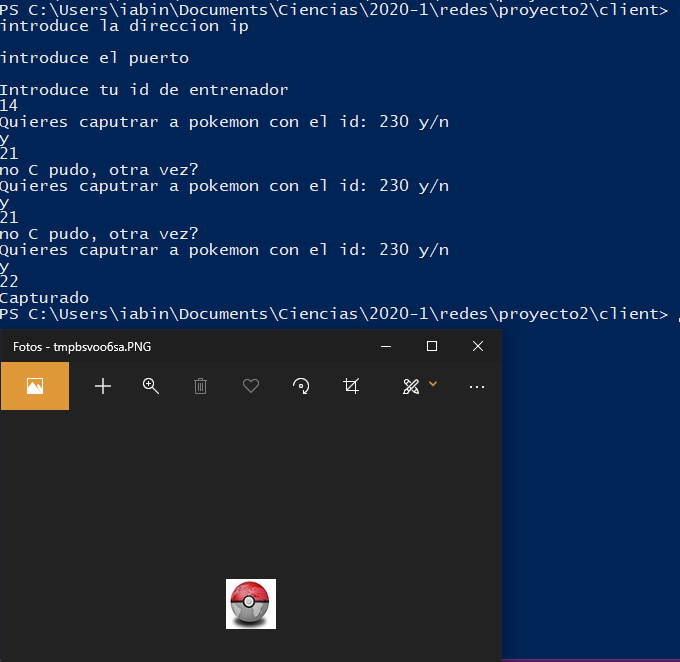
\includegraphics[scale=0.8]{casi.PNG}
    
    \item Las capturas se guardarán en la base de datos y para poder acceder a ellas tenemos que llamar en el intérprete cargar el script db.py en la carpeta server y ejecutar la función selectCaptures(), te mostrará el pokemonId y el id de usuario
    \\\\
    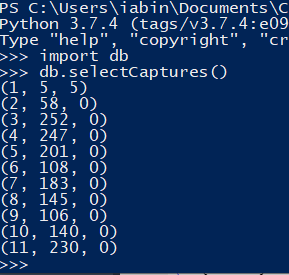
\includegraphics[scale=0.8]{db.PNG}
    \item Lamentablemente no se pudo interceptar los datos en wireshark
    debido a que no se puede interceptar localhost con wireshark en windows, pero viendo la implementación se puede ver los códigos que envía y recibe.
    
  
\end{itemize}
 
\end{document}
